\section{Incompatibility with Suspension-Based Locking Protocols}
\label{sec:locking}

\emph{Binary semaphores}, i.e., suspension-based locks used to realize mutually exclusive access to shared resources, are a common source of self-suspensions in multiprocessor real-time systems. When a task tries to use a resource that has already been locked, it self-suspends until the resource becomes available. Such self-suspensions due to lock contention, just like any other self-suspension, result in deferred execution and thus can detrimentally affect a task's interference on lower-priority tasks. It may thus seem natural to apply the period enforcer  to control the negative effects of blocking-induced self-suspensions.\footnote{The use of  period enforcement in combination with suspension-based locks has indeed been assumed in prior work~\cite{Raj:91} and suggested as a potential improvement elsewhere~\cite{Lak:11,LNR:09}.} However, as we demonstrate with two examples, it is actually not safe to use the period enforcer in the presence of suspension-based locks.

\subsection{Combining Period Enforcement and Suspension-Based Locks}

Whenever a task attempts to lock a shared resource, it may potentially block and self-suspend. In the context of the multi-segmented self-suspending task model, each lock request hence marks the beginning of a new segment.

The period enforcer algorithm may therefore be applied to determine the eligibility time of each such segment (which, again, all start with a critical section). There is, however, one complication: when does a task actually \emph{acquire} a lock? That is, if a task's execution is postponed due to the period enforcement rules, at which point is the lock request processed, with the consequence that the resource becomes unavailable to other tasks? 

There are two possible interpretations of how period enforcement and locking rules may interact. Under the \textbf{first interpretation}, when a task requires a shared resource, which implies the beginning of a new segment, its lock request is processed \emph{only when its new segment is eligible for execution}, as determined by the period enforcer algorithm. Alternatively, under the \textbf{second interpretation}, a task's request is processed \emph{immediately} when it requires a shared resource.

As a consequence of the first rule, a task may find a required shared resource unavailable when its new segment becomes eligible for execution even though the resource was available when the prior segment finished.  As a consequence of the second rule, a shared resource may be locked by a task that cannot currently use the resource  because the task is still ineligible to execute.

We believe that the first interpretation is the more natural one, as it does not make much sense to allocate resources to tasks that cannot yet use them. However, for the sake of completeness, we show that either interpretation can lead to deadline misses even if the task set is trivially schedulable without any enforcement.

\subsection{Case 1: Locking Takes Effect at Earliest Segment Eligibility Time}
In the following example, we assume the first interpretation, i.e., that the processing of lock requests is delayed until the point when a resuming segment would no longer be subject to any delay due to period enforcement. We show that this interpretation leads to a deadline miss in a task set that would otherwise be trivially schedulable.

Consider the following simple task set consisting of two tasks on two processors that share one resource. Task $\tau_1$, on processor~1, has a total execution cost of $C_1 = 4$ and a period and deadline of $T_1 = D_1 = 8$. After one time unit of execution, jobs of $\tau_1$ require the shared resource for two time units. $\tau_1$ thus consists of two segments with costs $C_1^1 = 1$ and $C_1^2 = 3$. Task $\tau_2$, on processor~2, has the same overall WCET ($C_2 = 4$), a slightly shorter period ($T_2 = D_2 = 7$), and requires the shared resource for one time unit after \emph{two} time units of execution ($C_2^1 = 2$ and $C_2^2 = 2$). Without period enforcement (and under any reasonable locking protocol), the task set is trivially schedulable because, by construction, any job of $\tau_1$ incurs at most one time unit of blocking, and any job of $\tau_2$ incurs at most two time units of blocking.

In contrast, with period enforcement, deadline misses are possible.
Figure~\ref{fig:locking-alt1} depicts a schedule of the two tasks assuming periodic job arrivals and use of the period enforcer algorithm. We focus on the eligibility times $ET_{2,1}^2,ET_{2,2}^2,ET_{2,3}^2,\ldots$ of the second segment of $\tau_2$.

\begin{figure}[t]
  \centering
  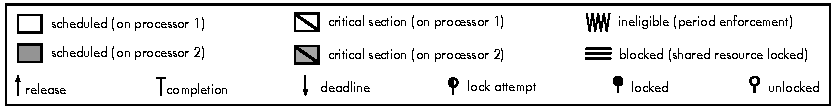
\includegraphics[scale=1]{../figures/locking/legend.pdf}
  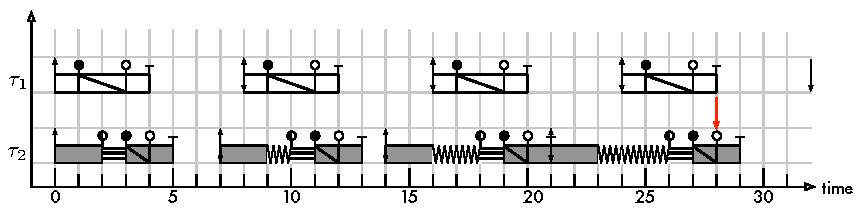
\includegraphics[scale=1]{../figures/locking/sched-locking-alt1.pdf}
  \caption{Example schedule of two tasks $\tau_1$ and $\tau_2$ on two processors sharing one lock-protected resource. The example assumes that lock requests take effect only when the critical section segment  becomes eligible to be scheduled according to the rules of the period enforcer algorithm. Under this interpretation, the fourth job of task $\tau_2$ misses its deadline at time $28$.}
  \label{fig:locking-alt1}
\end{figure}


Since $\tau_2$'s first job requests the shared resource only after two time units of execution, it is blocked by $\tau_1$'s critical section, which commenced at time $1$. At time $3$, $\tau_1$ releases the shared resource and $\tau_2$ consequently resumes (i.e., $a^2_{2,1} = 3$). According to the period enforcer rules~\cite{Raj:suspension1991}, the second segment is immediately eligible because, according to Equation~\ref{eq:ET-def} (in Section~\ref{sec:unschedulable}),
\begin{align*}
	ET_{2,1}^2 & = \max\left(ET_{2,0}^2 + T_2,\ \mathit{busy}(\tau_2, a^2_{2,1})\right) =\max(-T_2 + T_2,\ 3) = 3.
\end{align*}
(Recall that $ET_{2,0}^2 = -T_2$, and interpret $\mathit{busy}(\tau_2, a^2_{2,1})$ with respect to $\tau_2$'s processor.)


At time $7$, the second job of $\tau_2$ is released. Its first segment ends at time $9$. However, its second segment is not eligible to be scheduled before time $10$ since $ET_{2,2}^2 \geq ET_{2,1}^2 + T_2 = 3 + 7 = 10$. At time $9$, the second job of $\tau_1$, released at time $8$, can thus lock the shared resource without contention. Consequently, when $\tau_2$'s request for the shared resource takes effect at time $10$, the resource is no longer available and $\tau_2$ must wait until time $a^2_{2,2} = 11$ before it can proceed to execute. We thus have
\begin{align*}
	ET_{2,2}^2 & = \max\left(ET_{2,1}^2 + T_2,\ \mathit{busy}(\tau_2, a^2_{2,2})\right) =\max(10,\ 11) = 11.
\end{align*}

The third job of $\tau_2$ is released at time $14$. Its first segment ends at time $16$, but since $ET_{2,3}^2 \geq ET_{2,2}^2 + T_2 = 11 + 7 = 18$, the second segment may not commence execution until time~$18$ and the shared resource remains available to other tasks in the meantime. The third job of $\tau_1$ is released at time $16$ and acquires the uncontested shared resource at time $17$. Thus, the segment of $\tau_2$ cannot resume execution before time $a^2_{2,3} = 19$. Therefore
\begin{align*}
	ET_{2,3}^2 & = \max\left(ET_{2,2}^2 + T_2,\ \mathit{busy}(\tau_2, a^2_{2,3})\right) =\max(18,\ 19) = 19.
\end{align*}

The same pattern repeats for the fourth job of $\tau_2$, released at time $21$: when its first segment ends at time $23$, the second segment is not eligible to commence execution before time $26$ since $ET_{2,4}^2 \geq ET_{2,3}^2 + T_2 = 19 + 7 = 26$. By then, however, $\tau_1$ has already locked the shared semaphore again, and the second segment of the fourth job of $\tau_2$ cannot resume before time $a^2_{2,4} = 27$, at which point
\begin{align*}
	ET_{2,4}^2 & = \max\left(ET_{2,3}^2 + T_2,\ \mathit{busy}(\tau_2, a^2_{2,4})\right) =\max(26,\ 27) = 27.
\end{align*}
However, this leaves insufficient time to meet the job's deadline: as the second segment of $\tau_2$ requires $C_2^2 = 2$ time units to complete, the job's deadline at time~$28$ is  missed.

By construction, this example does not depend on a specific locking protocol; for instance, the effect occurs with both the MPCP~\cite{Ra:90} (based on priority queues) and the FMLP~\cite{BLBA:07,BA:08} (based on FIFO queues).  The corresponding response-time analyses for both protocols~\cite{Br:13,LNR:09} predict a worst-case response time of $6$ for task $\tau_2$ (i.e., four time units of execution, and at most two time units of blocking due to the critical section of $\tau_1$). 
This demonstrates that, under the first interpretation, adding period enforcement to suspension-based locks invalidates existing blocking analyses. Furthermore, it is clear that the devised repeating pattern can be used to construct schedules in which the response time of $\tau_2$  grows beyond any given implicit or constrained deadline.

Next, we show that the second interpretation can also lead to deadline misses in otherwise trivially schedulable task sets.

\subsection{Case 2: Locking Takes Effect Immediately}
 From now on, we assume the second interpretation: all lock requests are processed immediately when they are made, even if this causes the shared resource to be locked by a task that is not yet eligible to execute according to  the rules of the period enforcer algorithm. We construct an example in which a task's response time grows with each job until a deadline is missed.

To this end, consider two tasks with identical parameters hosted on two processors. Task $\tau_1$ is hosted on processor~1; task $\tau_2$ is hosted on processor~2. Both tasks have the same period and relative deadline $T_1 = T_2 = D_1 = D_2 = 8$ and the same WCET of $C_1 = C_2 = 4$. They both access a single shared resource for two time units each per job. Both tasks request the shared resource after executing for \emph{at most} one time unit. They both thus have two segments each with parameters $C_1^1 = C_2^1 = 1$ and $C_1^2 = C_2^2 = 3$. 

The example exploits that a job may require \emph{less} service than its task's specified WCET. To ensure that the shared resource is acquired in a certain order, we assume the following deterministic pattern of the actual execution times. Let $\epsilon$ be an arbitrarily small, positive real number with $\epsilon <1$. 
\begin{itemize}
	\item The first segment of even-numbered jobs  of $\tau_1$ executes for only $1-\epsilon$ time units.
	\item The first segment of odd-numbered jobs of $\tau_2$ executes for only $1-\epsilon$ time units.
%	the \nth{1}, \nth{3}, \nth{5}, \ldots, $(2i-1)$\xth job of , $\forall i=1,2,\ldots$.
%	the \nth{2}, \nth{4}, \nth{6}, \ldots, $(2i)$\xth jobs, $\forall i=1,2,\ldots$.
	\item All other segments execute for their specified worst-case costs.
\end{itemize}
Figure~\ref{fig:locking-alt2} shows an example schedule assuming periodic job arrivals.


At time $1-\epsilon$, the first job of $\tau_2$ acquires the shared resource because $\tau_1$ does not issue its request until time $1$. Consequently, $\tau_1$ is blocked until time $a^2_{1,1} = 3 - \epsilon$, and we have
\begin{align*}
	ET_{1,1}^2 & = \max\left(ET_{1,0}^2 + T_1,\ \mathit{busy}(\tau_1, a^2_{1,1})\right) =\max(-T_1 + T_1,\ 3 - \epsilon) = 3 - \epsilon
\\ \intertext{and}
	ET_{2,1}^2 & = \max\left(ET_{2,0}^2 + T_2,\ \mathit{busy}(\tau_2, a^2_{2,1})\right) =\max(-T_2 + T_2,\ 0) = 0.
\end{align*}

The roles of the second jobs of both tasks are reversed: since the second job of $\tau_1$ locks the shared resource already at time $9-\epsilon$, $\tau_2$ is blocked when it attempts to lock the resource at time~$9$. However, according to the rules of the period enforcer algorithm, the second segment of the second job of $\tau_1$ is not actually eligible to execute before time $11 - \epsilon$ since
\begin{align*}
	ET_{1,2}^2 & = \max\left(ET_{1,1}^2 + T_1,\ \mathit{busy}(\tau_1, a^2_{1,2})\right) =\max(3 - \epsilon + 8,\ 8) = 11 - \epsilon.
\end{align*}
Consequently, even though the lock is granted to $\tau_1$ already  at time $9-\epsilon$, the critical section is executed only starting at time $11 - \epsilon$, and $\tau_2$ is thus delayed until time $13 - \epsilon$. At time $13 - \epsilon$, $\tau_2$ is immediately eligible to execute since
\begin{align*}
	ET_{2,2}^2 & = \max\left(ET_{2,1}^2 + T_2,\ \mathit{busy}(\tau_2, a^2_{2,2})\right) =\max(0 + 8,\ 13 - \epsilon) = 13 - \epsilon.
\end{align*}

The third jobs of both tasks are released at time $16$. The roles are swapped again: because $\tau_2$'s first segment requires only $1-\epsilon$ time units of service, it acquires the lock at time $a^2_{2,3} = 17 - \epsilon$, before $\tau_1$ issues its request at time~$17$. However, according to the period enforcer algorithm's eligibility criterium, $\tau_2$ cannot actually continue its execution before time $21- \epsilon$ since
\begin{align*}
	ET_{2,3}^2 & = \max\left(ET_{2,2}^2 + T_2,\ \mathit{busy}(\tau_2, a^2_{2,3})\right) =\max(13- \epsilon + 8,\ 16) = 21- \epsilon.
\end{align*}
This, however, means that $\tau_1$ cannot use the shared resource before time $23 - \epsilon$, which leaves insufficient time to complete the second segment of $\tau_1$'s third job before its deadline at time $24$.
Furthermore, if both tasks continue the illustrated execution pattern, the period enforcer continues to increase their response times. As a result, the pattern may be repeated to construct schedules in which an arbitrarily large implicit or constrained deadline is violated.

As in the previous example,  the response-time analyses for both the MPCP~\cite{Br:13,LNR:09} and the   FMLP~\cite{Br:13} predict a worst-case response time of $6$ for both tasks (i.e., four time units of execution, and at most two time units of blocking). The example thus demonstrates that, if lock requests take effect immediately, then the period enforcer is incompatible with existing blocking analyses because, under the second interpretation, it increases the effective lock-holding times.


\begin{figure}[t]
  \centering
  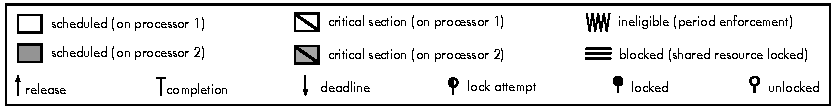
\includegraphics[scale=1]{../figures/locking/legend.pdf}
  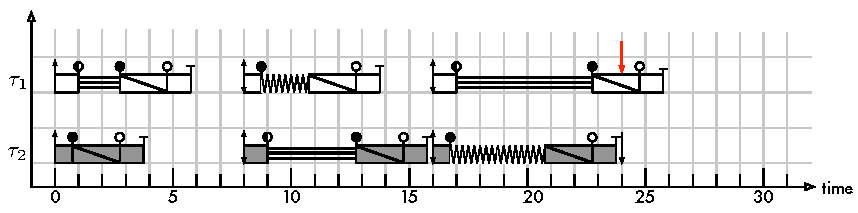
\includegraphics[scale=1]{../figures/locking/sched-locking-alt2.pdf}
  \caption{Example schedule of two tasks $\tau_1$ and $\tau_2$ on two processors sharing one lock-protected resource. The example assumes that lock requests take effect immediately, even if the critical section segment is not yet eligible to be scheduled according to the rules of the period enforcer algorithm. Under this interpretation, the third job of task $\tau_1$ misses its deadline at time $24$.}
  \label{fig:locking-alt2}
\end{figure}

\subsection{Discussion}

While it is intuitively appealing to combine period enforcement with suspension-based locking protocols, we observe that this causes non-trivial difficulties. In particular, our examples show that the addition of period enforcement invalidates all existing blocking analyses. They also suggest that devising a correct blocking analysis would be a substantial challenge due to the demonstrated feedback cycle between the period enforcer rules and blocking durations. 


Fundamentally, the design of the period enforcer algorithm implicitly rests on the assumption that a segment \emph{can} execute as soon as it is eligible to do so. In the presence of locks, however, this assumption is invalidated. As demonstrated, the result can be a successive growth of self-suspension times that proceeds until a deadline is missed.  The period enforcer algorithm, at least as defined and used in the literature to date~\cite{Raj:suspension1991,Raj:91}, is therefore incompatible with the existing literature on suspension-based real-time locking protocols (e.g., \cite{Raj:91,Lak:11,LNR:09,BLBA:07,Br:13}). 


Finally, it is worth noting that our examples can be trivially extended with lower-priority tasks to ensure that no processor idles before the described deadline misses occur. It is also not difficult to extend the second example with a task on a third processor such that all segments of $\tau_1$ and $\tau_2$ are separated by a non-zero self-suspension.
